\section{Einleitung}

Diese Ausarbeitung befasst sich mit dem Thema Smart Traffic. Im Modul Data Analytics des Masterstudiengangs Informatik an der HTWG sollen Möglichkeiten und Einsatzgebiete für das Complex Event Processing (CEP)  erarbeitet werden. Der Begriff \emph{Smart Traffic} bezeichnet dabei eine ereignisbasierte Mustererkennung im Straßenverkehr. Anhand einer Fallstudie werden in dieser Arbeit Szenarien für eine intelligente Steuerung des Verkehrs aufgezeigt. Abb. \ref{fig1} zeigt die Visualisierung  eines Straßenausschnitts, welcher für die Veranschaulichung der Smart Traffic Fallstudie verwendet wird. In diesem Verkehrskontext können nun fiktive Datenströme erzeugt werden, um bestimmte Verkehrssituationen zu simulieren. Eine Implementierung der CEP Engine ESPER ermöglicht die Erkennung und Verarbeitung von Verkehrsszenarien. Es werden Datenströme generiert, welche beispielsweise einen lokalen Unfall  repräsentieren. Die Mustererkennung von ESPER wird verwendet, um eine kluge (englisch smart) Umleitung des Verkehrs anzustoßen. Mit Hilfe einer WebUI kann der Verkehrsfluss gesteuert und verschiedene Verkehrsereignisse erzeugt und Kombiniert werden.

\begin{figure}[ht]
	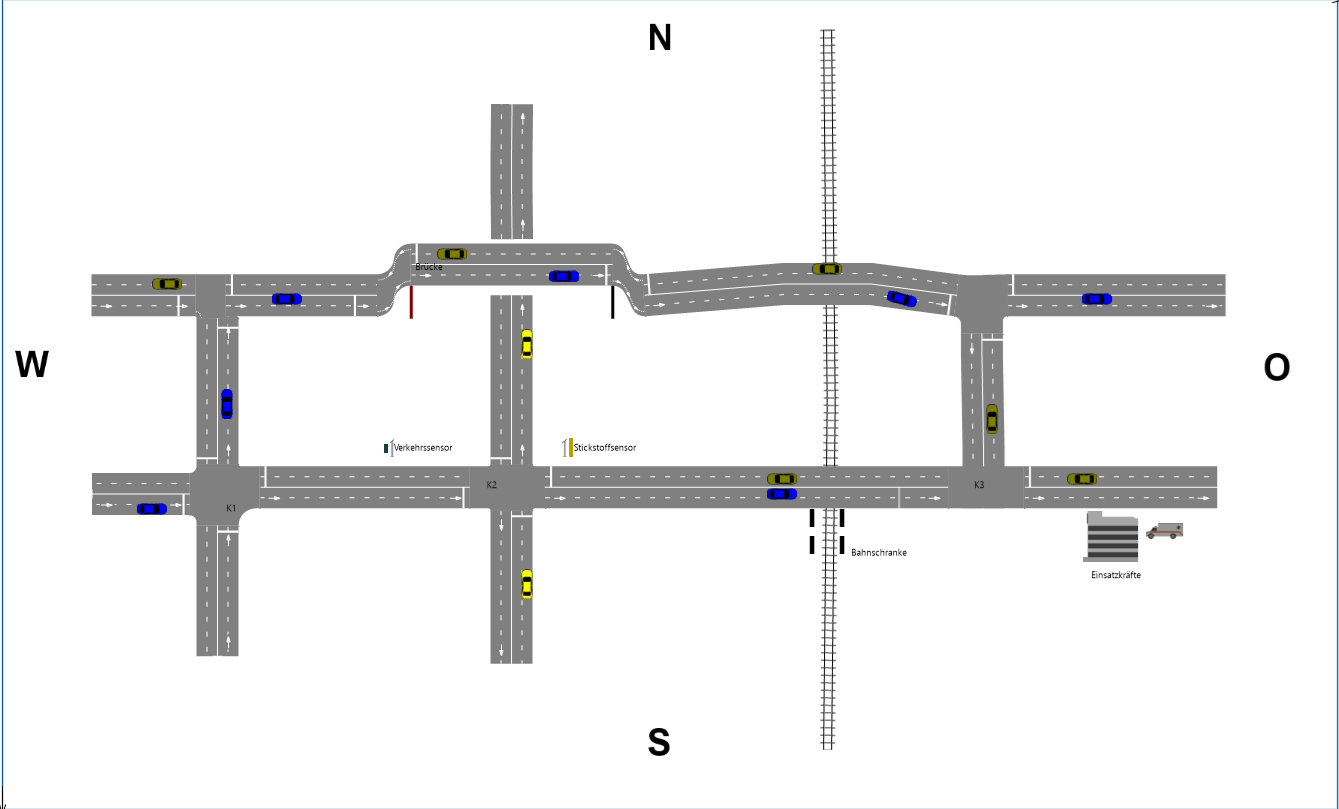
\includegraphics[width=\textwidth]{images/1_InitialStreetMap_Final.png}
	\caption{Straßenausschnitt der Fallstudie}
	\label{fig1}
\end{figure}




